\chapter{Bluetooth}
\label{chap:bluetooth}

Bluetooth is an IEEE standard(802.15.1+) registerd in 1999 and designed as a "wireless cable" more 
than a general-purpose wireless network. In fact, it is intended to be short-range, low-power, 
ubiquitous, and inexpensive, being roughly a wireless USB in capability and ubiquity.\\
Nowadays, the standard has quite evolved and it is possible to have a Bluetooth network.\\
\begin{figure}[H]
  \centering
  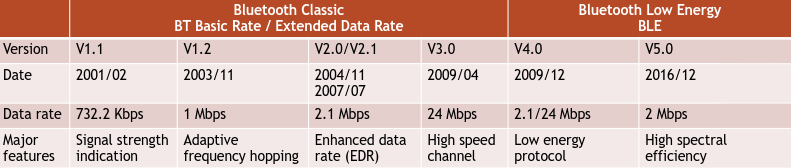
\includegraphics[width=0.7\textwidth]{img/wireless/bluetooth versions.png}
  \caption{Bluetooth versions}
\end{figure}
\begin{section}{Bluetooth networks}
  There are actually different types of Bluetooth networks.
  \begin{subsection}{Piconet}
    A piconet is a network of devices(ad-hoc) connected using Bluetooth technology withing a small area. 
    One device acts as the master and the other devices act as slaves. Up to seven slaves can be 
    connected to one master. The master controls the channel access of the slaves.\\
    The communication is strictly between a master and a slave at a time, no slave-to-slave communication
    is allowed.\\
    \begin{figure}[H]
      \centering
      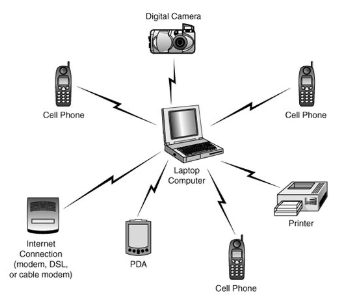
\includegraphics[width=0.4\textwidth]{img/wireless/piconet.png}
      \caption{A piconet bluetooth network}
    \end{figure}
  \end{subsection}

  \begin{subsection}{Scatternet}
    A scatternet is a network of piconets. A device in one piconet can be a slave in another piconet. 
    This allows the devices to communicate with each other even if they are not in the same piconet.\\
    One node can't be a master in two piconets at the same time and it may be a slave in one piconet and
    a master in another.\\
    \begin{figure}[H]
      \centering
      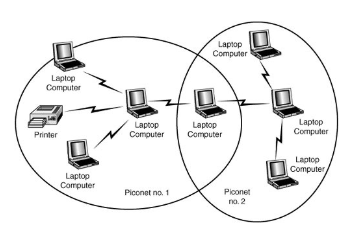
\includegraphics[width=0.4\textwidth]{img/wireless/scatternet.png}
      \caption{A scatternet bluetooth network}
    \end{figure}
  \end{subsection}

  \begin{subsection}{Personal Area Network}
    A Personal Area Network(PAN) is a network of devices within a range of 10 meters, using the bluetooth
    technology, in this case. It is meant to replace the cables between devices, like a wireless USB.\\
    It works in the 2.4-5 GHz frequency band and it is a low-power network, being able to transmit
    up to 3Mbps.\\
    This kind of network is an ad-hoc one, with a master controller and many clients, meaning that 
    it requires a polling mechanism to avoid collisions. It actually implements a TDM+FDM, with a 
    TDM slots of 625 ms and FDM over 79 channels in BT classic and 40 channels in BLE, while also 
    implmenting a frequency hopping mechanism.\\
    For energy saving, the devices can enter a low-power mode, where they can be woken up by the master
    controller. This network can also be \textit{self-assembling}, meaning that the devices can
    automatically connect to each other and set up a network.\\
    This requires means for authentication, authorization, confidentiality, and integrity.\\
  \end{subsection}
\end{section}

\begin{section}{Protocol stack}
  The protocol stack for the different versions of Bluetooth is shown in figure \ref{fig:bluetooth stack}.
  \begin{figure}[H]
    \centering
    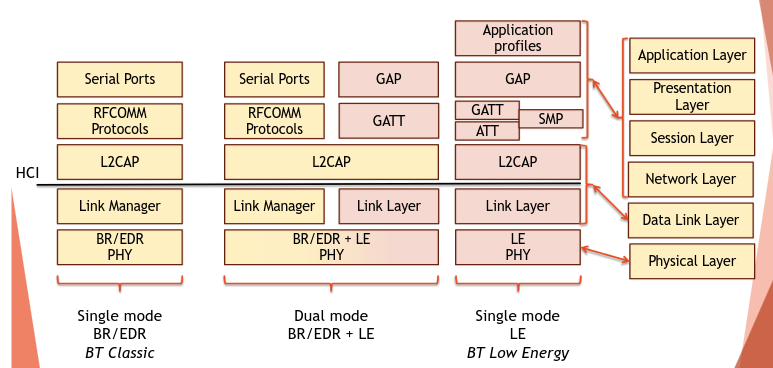
\includegraphics[width=0.7\textwidth]{img/wireless/bluetooth protocol tack.png}
    \caption{Bluetooth protocol stack}
    \label{fig:bluetooth stack}
  \end{figure}
  We will mainly focus on the more recent versions of Bluetooth(Low Energy).
  In bluetooth LE, there are 3 main specifications:
  \begin{itemize}
    \item the \textbf{core specifications}, which defines the architecture of the technology, the
      key features and the formal procedures, as well ad the protocols. 
    \item the \textbf{profiles}, which define the role of the device(client/server), its behavior and the
      transmitted data.
    \item the \textbf{services}, which define service group characteristics and descriptors,
      providing a formal description of the data exchanged between devices.
  \end{itemize}
  \begin{figure}[H]
    \centering
    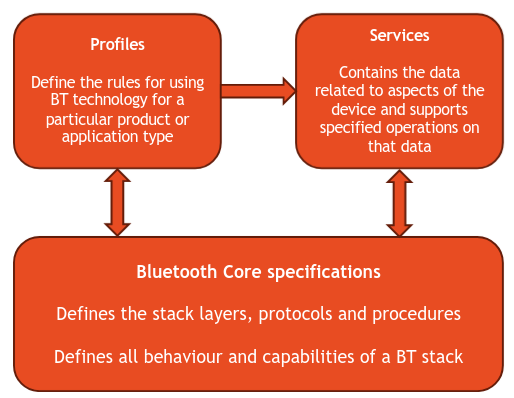
\includegraphics[width=0.5\textwidth]{img/wireless/bt specifivations.png}
    \caption{The 3 main specifications of Bluetooth LE}
  \end{figure}
  \begin{figure}[H]
    \centering
    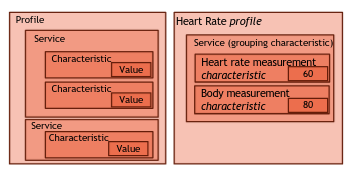
\includegraphics[width=0.5\textwidth]{img/wireless/bluetooth services format.png}
    \caption{An example of the data structure of some services}
  \end{figure}
  \begin{subsection}{The host stack}
    The host stack is the software stack that runs on the host device, which is the device that 
    controls the communication. 
    \begin{figure}[H]
      \centering
      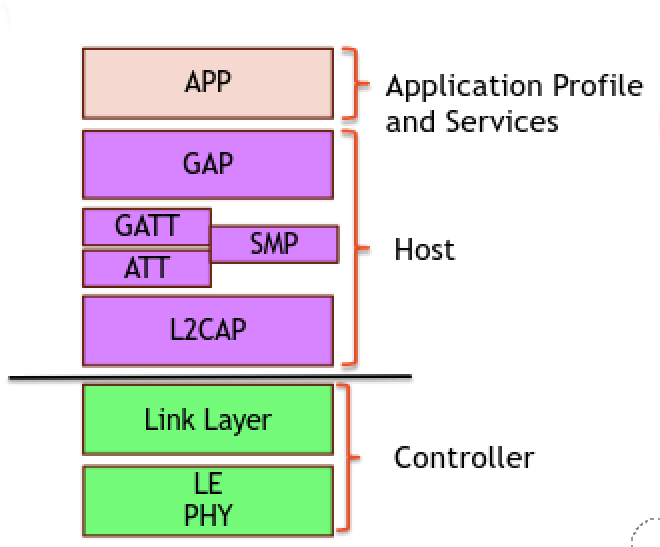
\includegraphics[width=0.4\textwidth]{img/wireless/bluetooth host stack.png}
      \caption{Bluetooth host stack}
    \end{figure}
    \begin{subsubsection}{Generic Access Profile}
      The Generic Access Profile(GAP) defines the roles, models, and procedures of a Bluetooth device.
      It provides communication channel between the devices, allowing them to:
      \begin{itemize}
        \item discover each other
        \item establish a link 
        \item terminate a link
        \item initialize the security features
        \item configure the device
      \end{itemize}
    \end{subsubsection}
    \begin{subsubsection}{Device states}
      The device can be in different states during the communication process:
      \begin{itemize}
      \item Standby: The device is in the initial idle state upon reset
      \item Advertiser: The device is advertising with specific data letting any initiating devices
        know that it is a connectible device. Messages contain the device address and some
        additional data, e.g. device name
      \item Scanner: When receiving the advertisement, the scanning device sends a scan request to
        the advertiser. The advertiser responds with a scan response. This process is called device
        discovery
      \item Initiator: When initiating, the initiator must specify a peer device address to which to
        connect. Suppose an advertisement is received matching the address of the peer device. In
        that case, the initiating device requests to establish a connection (link) with the
        advertising device specifying the Connection Parameters
      \item Slave/Master: Connection is formed. The device functions as a slave if the advertiser
        and a master if the initiator
      \end{itemize}
      \begin{figure}[H]
        \centering
        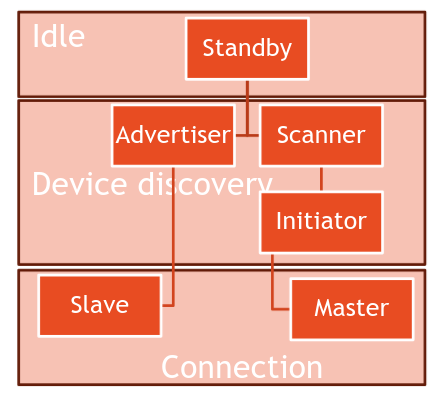
\includegraphics[width=0.4\textwidth]{img/wireless/bluethooth device states.png}
        \caption{Bluetooth device states}
      \end{figure}

    \end{subsubsection}
    \begin{subsubsection}{Generic attribute}
      The generic attribute(GATT) allows the devices to exchange data, providing data communication
      between two connected devices.\\ 
      Data is exchanged as a relationship data-attribute using a client-server model. The GATT-server
      accepts incoming commands and requests from a client and sends responses, indications, and notifications.
      The GATT-Client initiates commands and requests towards the server, receive responses, indications, and notifications.
    \end{subsubsection}

    \begin{subsubsection}{Attribute}
      The attribute level(ATT) transfers a single attribute data between the client and the server
      in the GATT-based profiles.\\
      Data can be accessed in different ways(read, wire, delete, \dots) and is organized in the form
      of attributes, each one having:
      \begin{itemize}
        \item an handle of 16-bits, which defines the type 
        \item an universally unique identifier(UUID)
        \item a value
        \item a set of permissions
      \end{itemize}
    \end{subsubsection}

    \begin{subsubsection}{L2CAP}
      L2CAP, or Logical Link Control and Adaptation Protocol, is the equivalent of the data link layer,
      which encapsulates data from the Bluetooth LE higher layers into the standard Bluetooth LE
      packet format for transmission according to the link configuration specified at the ATT and
      SMP layers.\\
      It provides means for:
      \begin{itemize}
        \item Protocol multiplexing
        \item Segmentation, and reassembly (SDU up to 64kB long)
        \item Retransmission
        \item Flow control
      \end{itemize}
      Under it, the HCI layer is responsible for the communication between the host and the
      controller, providing a command interface to the controller and a data interface to the host.

    \end{subsubsection}

  \end{subsection}
  \begin{subsection}{Service Discovery protocol}
    There's a middleware protocol that is not part of the Bluetooth stack, but it is used to discover
    the services provided by a device. This is the \textbf{Service Discovery Protocol}(SDP), which
    allows the devices to discover the services provided by another device, as well as their 
    associated parameters.\\
    It includes many phases, which are all optional.
    \begin{figure}[H]
      \centering
      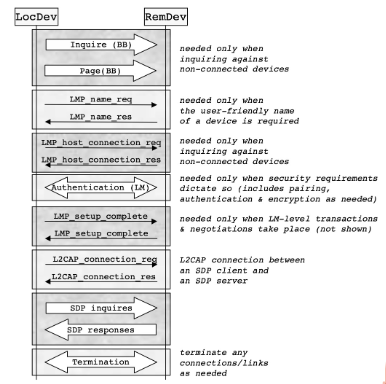
\includegraphics[width=0.5\textwidth]{img/wireless/bluetooth sdp.png}
      \caption{The messages exchanged during the SDP}
    \end{figure}
  \end{subsection}

  \begin{subsection}{The controller part}
    The controller part of the Bluetooth stack is the one that manages the physical layer and the
    link layer, allowing the host to communicate with the hardware.\\
    It is made up of 3 main components.
    \begin{subsubsection}{Host controller interface}
      The host controller interface(HCI) is the interface between the host and the controller, 
      providing a command interface to the controller and a data interface to the host.\\
      It defines a set of commands, events, and parameters that are used for the transmission and 
      the reception of data.\\
      When receiving packets from the controller, the HCI extracts raw data at the controller to
      send to the host.
    \end{subsubsection}
    \begin{subsubsection}{Link layer}
      The link layer is the one that manages the physical layer, providing the means for the 
      communication between the devices.\\
      It mainly manages the state of the link and defines the role of the device in the
      communication(Central, Pheripheral, Advertiser or Scanner).
    \end{subsubsection}
    \begin{subsubsection}{Physical layer}
      The physical layer is the one that manages the physical communication between the devices.
      It is responsible for the modulation, the frequency hopping, the power control, and the 
      encryption of the data.\\
      This layer quite differs between the different versions of Bluetooth( mainly BTL and BLE), but 
      the same principles are applied(Frequency hopping-Spread Spectrum).\\
      Both versions still use the same ISM(Industrial, Scientific, and Medical) band of 2.4 GHz to
      2.485 GHz, which is quite crowded, meaning that a lot of interference has to be managed.\\
      The first versions of Bluetooth(BR/EDR) use a frequency hopping mechanism with 79 channels of 
      1 MHz each, while more recent versions(BT 1.2+) uses adaptive frequency hopping(AHN) to avoid
      channels with interference, which is quite a bad idea in crowded scenarios.\\

      It implements forward error correction(FEC), which is a mechanism to correct errors in the
      data, using parity bits. FEC have 2 options: 
      \begin{itemize}
        \item 1/3 rate FEC, which means that each bit it sent 3 times, with 2 parity bits
        \item 2/3 rate FEC, which means that each sequence of 10 bits have 5 parity bits
          using a shortened Hamming code(10,15)
      \end{itemize}
      The standard also allows for the implementation of retransmission
      and automatic repeat request(ARQ) mechanisms, while also providing means for CRC and
      awcknowledgments.\\
      It also provides means for flushing the packets that are waiting an awcknowledgment, which
      can be useful in some cases, like audio streams.\\

      As for frequency modulation, the standard uses GFSK(Gaussian Frequency Shift Keying) for the
      data, forming a phase shift to encode the data.\\
      This schema provide a basic rate of 1Mbps, which can be increased doing differential quadrature
      phase shift keying(DQPSK) or Key Shift Keyring(PSK) to 3Mbps.\\

      Bluetooth is also able to use more frequency space than needed for the data rate, to spread the
      signal and make it more resilient to noise and interference. This is called spread spectrum
      and it is implemented using frequency hopping(could also have used CMDA).\\
      Frequency hopping is exactly what it sounds like: a channel is divided into smaller ones, and 
      for each time slot, the device changes the channel. 

      \begin{figure}[H]
        \centering
        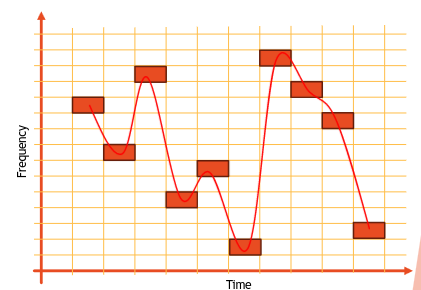
\includegraphics[width=0.5\textwidth]{img/wireless/frequency hopping.png}
        \caption{Bluetooth frequency hopping}
      \end{figure}
    This technique needs means for synchronization between the devices, which is done using a
    pre-detemined sequence of channels or announced by the master.\\

    A clock 312.5 $\mu$s long, dictated by the master, which is shared with the slaves.
    Two ticks can be grouped in a slot, which can be grouped, in a pair of 2, to form a slot pair,
    where the master send in the even slots and the slaves in the odd ones.\\
    Packets can be sent in 1, 3 or 5 slots.

    \end{subsubsection}

  \end{subsection}
\end{section}

\begin{section}{Bluetooth Frames}
  The structure of a Bluetooth frame is shown in figure \ref{fig:bluetooth frame}, for both 
  the standard and the enhanced data rate(EDR) versions.\\
  First of all, an access code of 72 bits is preset, which is used to synchronize the devices and
  identify the channel between the master and the slave.\\
  Then, an header of 54 bits, which is made up of the following fields:
  \begin{itemize}
    \item the address, which defines who the device is in the piconet. It of 3 bits because bt
      classic can host at most 8($2^3$) devices
    \item the type, which defines the type of the packet
    \item the flow, which defines the flow of the packet, if the buffer is full, theb it is set to
      notify not to send more packets
    \item the ARQN, which is the acknowledgment bit 
    \item the SEQN, which is the sequence number of 1 bit, because stop-and-wait ARQ is used and
      only need 1 bit
    \item the CRC, which is the cyclic redundancy check of 8 bits
  \end{itemize}
  If you sum up the bits, you don't get 53, but 18, because the header is sent 3 times.\\
  The payload can be up to 2744 bits long. In BT classic, everything is transmitted at the basic
  rate of 1Mbps, wheres in EDR, the header is transmitted at the basic rate, while the payload can 
  be transmitted at 2 or 3 Mbps, allowing to put up to 8184 bits in the payload. To accommodate the
  switch in the data rate, after the header a guard time equivalent of 16 bits is inserted.\\
  The whole transmission can be done in 675 $\mu$s that can be accommodated in 5 slots. If the
  packet is smaller, some padding could be added to fill the slot.\\

  \begin{figure}[H]
    \centering
    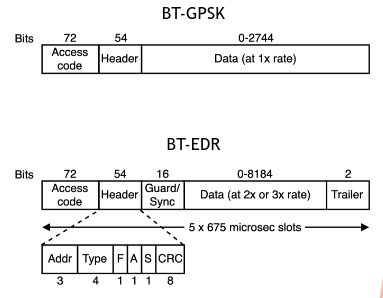
\includegraphics[width=0.5\textwidth]{img/wireless/bluetooth frame.png}
    \caption{The structure of a Bluetooth frame}
    \label{fig:bluetooth frame}
  \end{figure}
  \begin{subsection}{BLE frame structure}
    The structure of a BLE frame is similar to the one of the standard Bluetooth, but the frames are
    distinguished into two kinds: advertisement and data packets. The first ones travels trough 3
    dedicated advertisement channels, while the second ones travels through the remaining 36 data
    channels.\\
    The general structure of a BLE frame is shown in figure \ref{fig:ble frame}, and is the
    following:
    \begin{itemize}
      \item a 8 bit preamble used for synchronization
      \item a 4 byte access address, used to identify the connection and randomly generated per the
        BLE connection. Collisions in the access address are possible with probability $2^{-32}$.
        There's a unique broadcast access address that is used for advertisement packets, that is
        0x8E89BED6
      \item a 3 byte CRC
    \end{itemize}
    \begin{figure}[H]
      \centering
      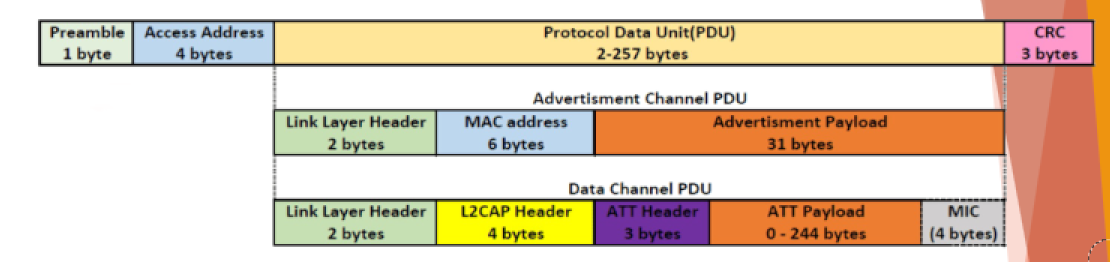
\includegraphics[width=0.7\textwidth]{img/wireless/BLE frame.png}
      \caption{The structure of a BLE frame}
      \label{fig:ble frame}
    \end{figure}
  \end{subsection}
  
  \begin{subsection}{Bluetooth Addresses}
    Addresses in Bluetooth are very similar to the ones in Ethernet, being unique and 48 bits long.
    The address is divided in 3 parts:
    \begin{itemize}
      \item NAP - Non-significant Address Part (2 bytes). Used in Frequency Hopping Synchronization
        frames
      \item  UAP - Upper Address Part (1 byte). Used for seeding in various Bluetooth specification
        algorithms
      \item  LAP - Lower Address Part (3 bytes). Allocated by the vendor. The LAP value uniquely
        identifies a Bluetooth device as part of the Access Code in every transmitted frame
    \end{itemize}
    \begin{figure}[H]
      \centering
      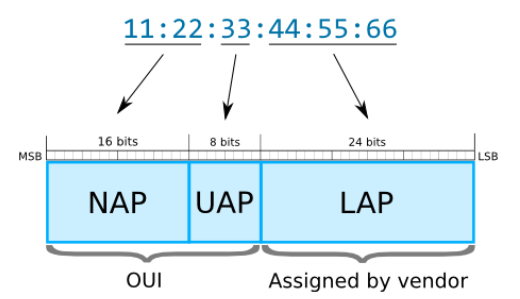
\includegraphics[width=0.5\textwidth]{img/wireless/bt addresses.png}
      \caption{Bluetooth addresses}
    \end{figure}
  \end{subsection}
\end{section}

\begin{section}{Bluetooth security}
  Bluetooth offers some security services, like:
  \begin{itemize}
    \item Authentication, but not user authentication
    \item Authorization
    \item Confidentiality
  \end{itemize}
  In fact, the bluetooth security model inclues five distinct security features:
  \begin{itemize}
    \item Pairing, the initial process of establishing one or more shared secret key between two
      devices
    \item Bonding, the process of storing the keys in the devices, so that they don't have to be
      established again
    \item Device Authentication, the process of verifying if two devices have the same key
    \item Encryption, to provide confidentiality
    \item Message integrity
  \end{itemize}
  \begin{subsection}{BT classic}
    Bluetooth classic uses a 4-to-6-digit PIN to establish a connection and authenticate the
    devices, which the two device agree on.\\

    The keys are generated during the legacy pairing process, using the SAFER+ algorithm, which is
    a symmetric block cipher. The key is with a custom algoritm based on that one, called E21 and
    E22, and use E1 as the authentication protocol. Those algorithm were chosen because they were
    open and free to use.\\
    The encryption mechanism is based on the E0 stream cipher, which is derived from the
    Massey-Rueppel algorithm.\\
    Integrity is not really provided, because no cryptographic integrity is provided, but a CRC is
    used to check the integrity of the data.
    \begin{subsubsection}{Pairing}
      Before 4.2, the pairing process was quite simple, with the devices exchanging the PIN and
      generating the keys.\\
      For this purposes, SHA-256, HMAC-SHA-256 and P-256 elliptic curve were used.\\
      Because permission from the user is required, there are 4 main association models:
      \begin{itemize}
        \item Just Works, where the devices exchange the keys without any user interaction
        \item Numeric Comparison, where the devices exchange a number that the user has to compare
        \item Passkey Entry, where the user has to enter a passkey
        \item Out of Band, where the devices exchange the keys using a different channel
      \end{itemize}
      In version 4.2 or higher, a new standard was proposed, upgrading the secure simple pairing
      to utilize the P-256 elliptic curve, HMAC-SHA-256, AES-CTR and adding message integrity via 
      AES-CCM.
    \end{subsubsection}
  \end{subsection}
  \begin{subsection}{Security Manager Protocol}
    Before BLE, the security properties were scattered across the whole protocol stack, but in BLE
    a new layer was introduced, the Security Manager Protocol(SMP), which is responsible for the
    security of the communication.\\

    \begin{figure}[H]
      \centering
      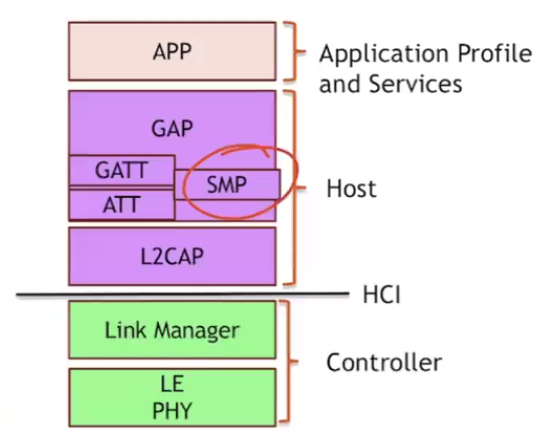
\includegraphics[width=0.4\textwidth]{img/wireless/security manager protocol.png}
      \caption{The security manager protocol in the Bluetooth stack}
    \end{figure}
    Fundamentally, the SMP is a p2p protocol used to generate the encryption keys and the identity
    keys and also manage their storage. The whole protocol operates over L2CAP to create a dedicated
    and fixed channel.\\
    It is also responsible to support random address generation and resolution, which is a privacy
    feature that allows the devices to change their address to avoid tracking.

  \end{subsection}
  \begin{subsection}{Bluetooth Security Levels}

    Security levels refer to a combination of security attributes and requirements that determine
    the level of protection provided by a Bluetooth connection. There are four main security levels
    in Bluetooth:

    \begin{itemize}
      \item No security: This level provides no security and is susceptible to any kind of attack.
      \item Unauthenticated pairing with Encryption: This level uses AES-CMAC encryption to protect
        data, but does not require authentication during pairing. This makes it vulnerable to
        man-in-the-middle (MITM) attacks.
      \item Authenticated Pairing with Encryption: This level requires authentication during pairing
        and uses encryption to protect data. This is a more secure option than level 2.
      \item Authenticated LE Secure Connections Pairing with Encryption Using a 128-Bit Strength
        Encryption Key: This is the most secure level and offers the highest level of protection. It
        uses ECDHE (Elliptic Curve Diffie-Hellman) encryption and requires authentication during
        pairing.
    \end{itemize}
  \end{subsection}
  \begin{subsection}{Bluetooth Security Modes}
    Security levels refer to a combination of security attributes and requirements that determine the level of protection provided by a Bluetooth connection. There are four main security levels in Bluetooth:

    \begin{itemize}
      \item Security Level 1: No security  - This level provides no security and is susceptible to
        any kind of attack.
      \item Security Level 2: Unauthenticated pairing with Encryption - This level uses AES-CMAC
        encryption to protect data, but does not require authentication during pairing. This makes
        it vulnerable to man-in-the-middle (MITM) attacks.
      \item Security Level 3: Authenticated Pairing with Encryption - This level requires
        authentication during pairing and uses encryption to protect data. This is a more secure
        option than level 2.
      \item Security Level 4: Authenticated LE Secure Connections Pairing with Encryption Using a
        128-Bit Strength Encryption Key - This is the most secure level and offers the highest level
        of protection. It uses ECDHE (Elliptic Curve Diffie-Hellman) encryption and requires
        authentication during pairing.
    \end{itemize}

  \end{subsection}
  
  \begin{subsection}{Pairing}
    Pairing is the process of establishing a secure connection between two Bluetooth devices, and
    usually involves the establishment of encryption keys that are used to protect the data.
    Those keys will also be used to verify signed data and perform random address resolution.\\

    As previously stated, the pairing move from the legacy version, which was based on a pin of 4 or 
    6 digits, to a new version, the Secure Simple Pairing, after release 4.2, which tries to make
    the pairing procedure simpler to the user while also improving the security.\\
    This was necessary because the old pairing method was very vulnerable to brute force attacks,
    because the PIN was very short.\\
    The new version goals were also to provide protection against passive eavesdropping and active
    MITM attacks.\\
    The obvious solution is to use public key cryptography to avoid brute force attacks, but this
    would mean that MITM attacks would still be possible. For this reason an challenge based on an
    out-of-band secret that the attacker doesn't know is used.\\
    This is done in 2 ways:
    \begin{itemize}
      \item Numerical comparison, where the devices shows on screen a number and the users have to
        make sure that those numbers are the same
      \item Passkey entry, where the user has to enter the pin
    \end{itemize}
    For compatibility reasons, a 6-digit number is used.

    As you can see in figure \ref{fig:pairing}, the pairing process is made up of 3 main phases.

    \begin{figure}[h]
      \centering
      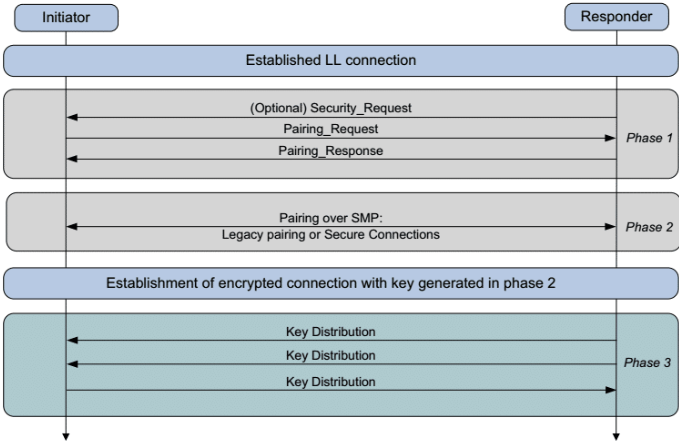
\includegraphics[width=0.5\textwidth]{img/wireless/bt pairing overview.png}
      \caption{General overview of the pairing process}
      \label{fig:pairing}
    \end{figure}

    \begin{subsubsection}{Phase 1: Feature Exchange}
      In this phase, the devices exchange their features, like the I/O capabilities, the out-of-band
      data, the authentication requirements, \dots\\
      This is done trough a pairing request, with code 0x01, and a pairing response, with code 0x02.
      In the same message, the security requirements of the link are also exchanged, in particular,
      if the key should be stored to be reused later(bonding flag), if MITM protection is required,
      ,if secure connection should be used and if passkey entry protocol is required.\\
      The maximum encryption key size is also exchanged, which could be from 7 to 16 bytes.\\
      \begin{figure}[H]
        \centering
        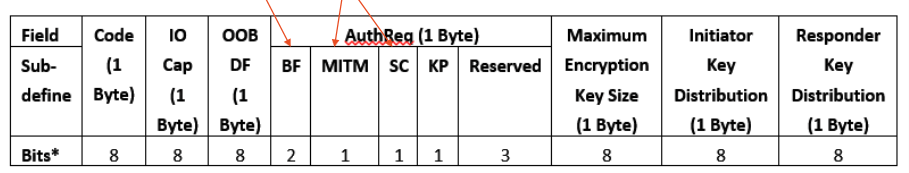
\includegraphics[width=0.7\textwidth]{img/wireless/bt feature exchange.png}
        \caption{Feature exchange}
      \end{figure}
    \end{subsubsection}

    \begin{subsubsection}{Phase 2: Pairing}
      The second phase varies according to the version of bluetooth used, it could be the legacy
      pairing or the new Secure Connection. To choose between the two, a bit have to be set in the
      previous phase, and both device must support it and agree on it.\\
      Authentication in Secure Connection is carried out via ECDH(Elliptic Curve Diffie-Hellman) and
      challenge response authentication. The 6-digit pin is then generated from both public keys and
      the nonces.\\
      You could have noticed that this process is vulnerable to MITM attacks, buts this is not true
      because of the order of the messages, in fact the challenge is computed from a nonce, which is
      sent to the other party only after the other nonce has been received.\\
      \begin{figure}[H]
        \centering
        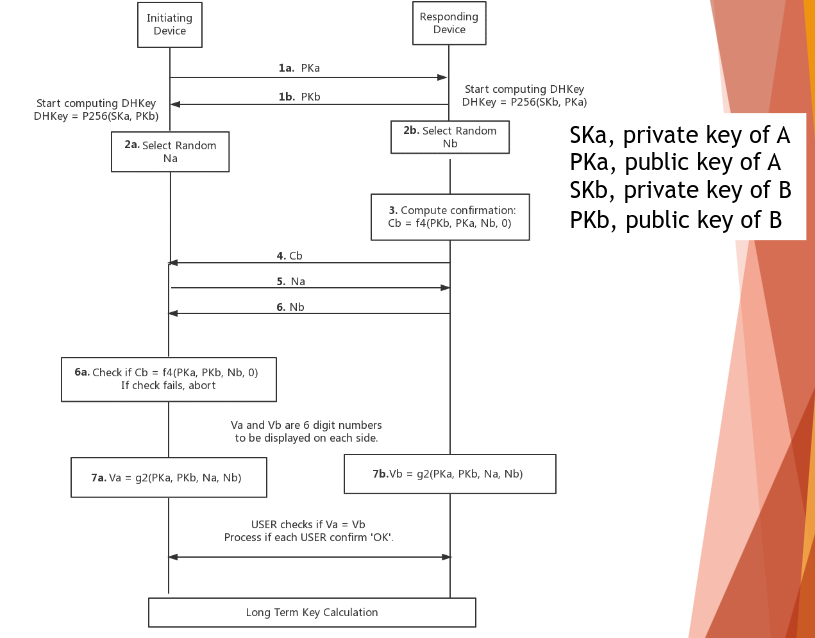
\includegraphics[width=0.7\textwidth]{img/wireless/bt pairing dhke.png}
        \caption{The DH key exchange performed in the pairing phase}
      \end{figure}
      Furthermore, if MITM protection has been requested, the user is involved in an interactive
      procedure by which the user confirms the pairing. The devices can then authenticate each other
      using a procedure that involves the private keys of the two devices. Long Term Key (LTK) is
      calculated (and other keys as well if needed).\\

    \end{subsubsection}

    \begin{subsubsection}{Phase 3: Key Distribution}
      The link is encrypted with a session key derived from LTK, and keys of types established in
      phase 1 are distributed. Sometimes this is a unidirectional process from Peripheral to Central
      and sometimes it is bi-directional.
    \end{subsubsection}
  \end{subsection}
\end{section}

\begin{section}{Bluetooth Privacy}
  Bluetooth has some privacy issues, mostly because bt devices, like a smartphone are devices that
  people carry around with them all the time, and they can be used to track the user because they
  keep advertising their presence.\\
  A solution is to change the MAC address frequently enough to avoid tracking, but this is not
  a easy feat, because they are used to identify the device in the network.\\
  In practice, a series of random addresses are generated and used for a short period of time(15
  minutes is recommended) before rotating to a new one. This solve an issue but creates another one,
  because the pairing process is based on the MAC address. To solve this, a new feature was
  introduced, called Resolvable Private Address, which allow to create private addresses based on
  the device IRK(Identity Resolving Key), exchanged during the bonding process.

  \begin{subsection}{Bluetooth Privacy Modes}
    Two modes of privacy are available:
    \begin{itemize}
      \item Device Privacy Mode: This mode focuses on the privacy of the device itself. It will
        accept advertising packets from other devices regardless of their Identity Resolving Key
        (IRK) distribution.
      \item Network Privacy Mode: This mode prioritizes the privacy of other devices on the network.
        It will only accept advertising packets that meet specific criteria:
        \begin{itemize}
          \item Packets must use the private addresses of the sending devices.
          \item Packets must be verifiable.
        \end{itemize}
        It will not accept packets containing the Identity Address of devices that have not distributed their IRK.
    \end{itemize}
    In essence, device privacy mode prioritizes the device's ability to receive information, while network privacy mode prioritizes the privacy of other devices on the network.
  \end{subsection}

  \begin{subsection}{Device addresses}
    4 kinds of addresses are used in Bluetooth:
    \begin{itemize}
      \item Public addresses, which are fixed and never change for a device
      \item Random addresses, which don't need to be registered
      \item Static addresses, which ends with "11" and are randomly generated at each boot to
        uniquely identify the device in the piconet
      \item Private addresses, which are generated using the IRK and are used to avoid tracking
        \begin{itemize}
          \item Resolvable Private Address: a random sequence of 46 bits that ends with 00 and
            doesnt allow bonding
          \item Non-Resolvable Private Address: a random sequence of 46 bits that ends with 10 and
            allows bonding. Can be resolved only by trusted devices.
        \end{itemize}
    \end{itemize}

    \begin{subsubsection}{Resolvable private addresses}
      As you know, after pairing, during bonding phase the devices exchange and share keys,
      including the IRK, which allows the device to sign the address so that only devices that knows
      the IRK can resolve the address.\\

      The address is generated from a 22-bit random number and the IRK($h=hash(IRK,rand)$), which
      returns a 24-bit number. The address is then formed by the 24-bit number and the 22-bit
      random number, along with the trailing '10' bits.\\

      To verify the address, the device that wants to resolve it has to hash the IRK and the random
      number, which is extracted from the address itself, and compare the result with the address.
      If they match the address is resolved, otherwise it is not.\\

      \begin{figure}[H]
        \centering
        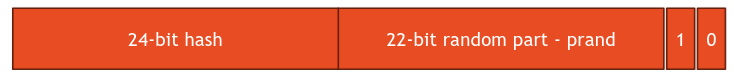
\includegraphics[width=0.6\textwidth]{img/wireless/resolvable private address.png}
        \caption{Structure of a resolvable private address}
      \end{figure}

    \end{subsubsection}
  \end{subsection}
\end{section}

\begin{section}{Bluetooth vulnerabilities}
  Multiple vulnerabilities have been discovered in Bluetooth over time.
  \begin{subsection}{Denial of service attacks}
    Just last year, it was found out that apple devices accepts advertising packets from any apple
    device witouth pairing. This means that by simple replaying or forging an advertising packet, an
    attacker could flood the device's screen with popups, effectively rendering the device unusable,
    or even crash the device.\\
    This is a very simple example of a denial of service attack, and in this case the damage is
    "limited", but in other cases, the attacker could have done more damage.\\
    Some other examples of DoS attacks are:
    \begin{itemize}
      \item Bluejack, which is a DoS attack that involves sending spam messages to a device
      \item Bluesnarf, which is a DoS attack that involves stealing data from a device exploiting a
        vulnerability in a file exchange protocol
    \end{itemize}
  \end{subsection}
  \begin{subsection}{MITM attacks}
    One of the reasons that the LE version was introduces was to avoid MITM attacks, which were
    possible because only the user has to be authenticated to the master, not the slave.\\
    As such, the BIAS attack was discovered, which allows an attacker to impersonate a device and
    establish a connection with another device, without knowing the long term key.\\
    \begin{figure}[H]
      \centering
      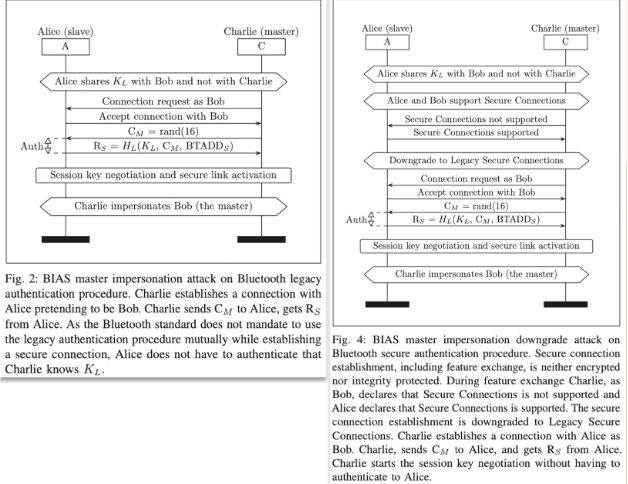
\includegraphics[width=0.7\textwidth]{img/wireless/bias attack.png}
      \caption{The BIAS attack}
    \end{figure}


  \end{subsection}

\end{section}

\begin{section}{Questions and answers}
  \begin{subsubsection}{Explain the main design goals for the Bluetooth technology and the technical
    constraints that guided the design}
    Origianlly, bluetooth was designed to be a "wireless cable", being short-ranged, low-power and
    with a limited troughput. It didnt require an infrastructure and would have been
    self-configuring.
    Some technical constraint made some decisions necessary:
    \begin{itemize}
      \item in mobile devices energy is a precious resource, making the standard low-power 
      \item bluetooth works on the 2.3Ghz spectrum, which is quite cramped, making the decision to
        be short ranged to avoid interference and save power obvious. This made frequency hopping
        necessary too.
      \item the auto-configuring feature was made necessary by the fact that not all devices have
        the i/o peripherals necessary to configure the infrastructure or connect to it 
    \end{itemize}
  \end{subsubsection}
  \begin{subsubsection}{Describe the Bluetooth network topologies and the role of nodes in each
    scenario}
    There are 3 main bt topologies:
    \begin{itemize}
      \item a piconet is a small bt network(up to 8 devices) in which a node acts as a master, while
        all the others are the slave devices. The master orchestrate all the ommunications, which
        are strictly between the master and a slave, one at the time.
      \item a scatternets is a bt network made up of many piconets. A device can be master in one
        and a slave in another one, but can't be a master in more than one. This allows nodes to
        communicate across piconets.
    \end{itemize}
  \end{subsubsection}
  \begin{subsubsection}{Describe the physical layer communication mechanisms implemented in
      Bluetooth BR/EDR and the differences since BLE was introduced: which frequency range does it
    use, which multiple access scheme does it use, which FEC/ARQ mechanism it provides, etc.}
  \end{subsubsection}
  \begin{subsubsection}{Describe what are the profiles, the services and the core specifications in
    Bluetooth}
    The core specifications defines the architecture of the technology, it's features, the protocols
    nad the formal procedures.\\
    The profiles defines the role of the device in the communication(if its a client or a server) as
    well as the transmitted data, while the services defines the service group characteristics,
    providing a formal description of the exchanged data. 
  \end{subsubsection}
  \begin{subsubsection}{Describe the Bluetooth device states (standby, advertiser, scanner,
      initiator, master, slave) and provide an example considering two devices that would like to
    interconnect}
    The states in which a bt device can be are:
    \begin{itemize}
      \item standby: the device has just boot up 
      \item advertiser: the device is advertising its presence to the neibouring devices, sending
        frames to inform that it is a connectible device, with some iformations such as the device
        address and its name
      \item scanner, the device is looking for connectible devices, listening to the advertisement
        packers and sending a scan request that will be responded to.
      \item initiator: a device request to enstablish a link with an advertisement device 
      \item slave and master: the devices are connected, and the initiator is the master
    \end{itemize}
  \end{subsubsection}
  \begin{subsubsection}{What are the functionalities of the Logical Link Control and Adaptation
    Layer Protocol (L2CAP) in Bluetooth?}
    The L2CAP protocol encapsulates data from the higher leves for transmission according to the
    link configuration. I multiplexes the higher level protocols, provides segmentaation and
    reassembnlation features, a retransmission mechanism an control flow.
  \end{subsubsection}
  \begin{subsubsection}{Describe the connection setting up process when there is a device in a
    discoverable state}
  \end{subsubsection}
  \begin{subsubsection}{Describe the CDMA mechanisms used in Bluetooth and compare it again simple
    FDMA and TDMA schemes}
  \end{subsubsection}
  \begin{subsubsection}{Why it is important to implement FEC schemes in BT? Which FEC protocols does
    the standard support? Does it support ARQ as well? Which type?}
    BT works over the 2.4GHz frequency band, which is quite crowded as its unlicensed, this means
    that a lot of interference is to be expected. A forward error correction schema is thus
    necessary to ensure the reliability of the communication.\\
    The standard supports 2 fec schemes:
    \begin{itemize}
      \item 1/3 FEC rate: each bit is send bit 3 times(1 data and 2 parity bits)
      \item 2/3 FEC rate: each sequence of 10 bits have 5 parity bits which ises a shortened hamming
        code 
    \end{itemize}
    BT supports arq but doesnt specify a standard to follow, it's up to the impelementation.
  \end{subsubsection}
  \begin{subsubsection}{Which security services does BT support? Which are the five distinct
    security models implemented in the standard?}
    BT supports as security services confidentiality, authentication and authorization. 
  \end{subsubsection}
  \begin{subsubsection}{Describe the four association models of Bluetooth}
  \end{subsubsection}
  \begin{subsubsection}{Describe the security levels and modes of BT}
  \end{subsubsection}
  \begin{subsubsection}{Describe the three phases of the pairing process}
  \end{subsubsection}
  \begin{subsubsection}{What are the goals of the legacy pairing and what are the weaknesses that
    make it a vulnerable protocol? How are these addressed in the Secure Simple Pairing protocol?}
  \end{subsubsection}
  \begin{subsubsection}{Detail the MITM attack that could be possible during the pair phase. How can
    this be avoided?}
  \end{subsubsection}
  \begin{subsubsection}{Describe the security features and the input/output capabilities exchanged
    during phase 1 of the pairing process – the feature exchange}
  \end{subsubsection}
  \begin{subsubsection}{Sketch the Elliptic Curve Diffie-Hellman authentication implemented in BT
    pairing}
  \end{subsubsection}
  \begin{subsubsection}{What are the privacy attacks one could build against a user with a BT
      device? How is this problem addressed? Describe the different MAC address types and detail how
    the resolvable private addresses work}
  \end{subsubsection}
  \begin{subsubsection}{Describe the bluejacking and bluesnarfing attacks}
  \end{subsubsection}
\end{section}
